% Created 2020-11-10 二 22:38
% Intended LaTeX compiler: xelatex
\documentclass[11pt]{report}
\usepackage{graphicx}
\usepackage{grffile}
\usepackage{longtable}
\usepackage{wrapfig}
\usepackage{rotating}
\usepackage[normalem]{ulem}
\usepackage{amsmath}
\usepackage{textcomp}
\usepackage{amssymb}
\usepackage{capt-of}
\usepackage{hyperref}
\author{曹嘉祺 PB18030874 化学与材料科学学院 有机化学系 \thanks{中国 安徽合肥 中国科学技术大学 Email: \href{mailto:mkq@mail.ustc.edu.cn}{mkq@mail.ustc.edu.cn}}}
\usepackage[scheme=plain]{ctex}
\usepackage{fontspec}
\setmainfont{更纱黑体 UI SC}
\hypersetup{colorlinks=true,linkcolor=blue}
\usepackage{longtable}
\date{\today}
\title{磁化率——络合物结构的测定}
\hypersetup{
 pdfauthor={曹嘉祺 PB18030874 化学与材料科学学院 有机化学系},
 pdftitle={磁化率——络合物结构的测定},
 pdfkeywords={},
 pdfsubject={},
 pdfcreator={Emacs 27.1 (Org mode 9.4)}, 
 pdflang={English}}
\begin{document}

\maketitle
\tableofcontents

\begin{abstract}
在文中首先介绍了磁介质在磁场中的磁化现象,然后通过对一些物质的磁化率的测定,求出未成对电子
数并判断络合物中央粒子的电子结构和成键模型,另外,用古埃磁天平在近似的条件下,根据居里—外斯定律
求出分子的磁矩及磁化率,进而根据未成对电子数来判断分子的成键结构。

\noindent\rule{\textwidth}{0.5pt}
\begin{itemize}
\item 关键词: 磁介质\quad 磁化率\quad 古埃磁天平\quad 居里—外斯定律
\end{itemize}
\end{abstract}




\begin{abstract}
Magnetization phenomenon having introduced that the magnetizable medium hits the
target in the magnetic field first in culture, and then by the admeasurement to a little matter
specific magnetization, ask out become the electron structure to the electron number and sigmic
judging complex compound central authority and become the key model , another, use Guai
magnetism balance under similar condition, regulation and the specific magnetization, are based
on the structure coming not to judge the molecular Cheng key twinning electron number then
according to the magnetism that this Curie outside law asks to produce a molecule.

\noindent\rule{\textwidth}{0.5pt}

\begin{itemize}
\item key words:  Magnetizable medium, Specific magnetization, Guai magnetism balance, This Curie outside law,
\end{itemize}
\end{abstract}
\part{前言}
\label{sec:orgda20aa6}
磁化率在判断物质分子中是否存在未成对电子及配合物结构类型等方面具有重要应用;
通过物质磁化率的测定来计算分子中未成对电子数是研究分子中成键情况的有效方法。络合
物电子结构的测定——古埃磁天平法(磁化率的测定)是比较简单,却能够得到物质结构很多
信息的一种方法。
本文将采用MB-1A型磁天平,通过很简便快速的方法,得到物质结构的信息。

\chapter{磁介质的磁化}
\label{sec:orgf990994}
    当磁介质放到场强为H的磁场中会产生附加的磁场H′,这种现象称为磁介质的磁化。
这时磁介质的磁感应强度为:
\[
B=H+H'=H+4\pi XH
\]
式中 X 为物质的体积磁化率,化学中常用克磁化率 X\textsubscript{m} 和摩尔磁化率 X\textsubscript{M} ,它们的定义为:
\[
X_{m}=X/\rho
\]
\[
X_{M}=MX/\rho
\]
式中 \rho为磁介质的密度,M 为克分子量。由于 X 是无量纲的量,故 X\textsubscript{m} 和 X\textsubscript{M} 的量纲为
cm\textsuperscript{3}/g 和cm\textsuperscript{3}/mol,式中如 H′ 和 H 同向则为顺磁物质,H′ 和 H 反向为逆磁质 H′ 和 H
不成正比,H′ 随 H 的增加而剧烈增加,当外磁场消失后这种物质的磁性并不消失,呈现滞
后的现象,则为铁磁质。
\chapter{原子分子的磁矩}
\label{sec:org39cd7e5}
   由于分子体系内有电子环形运动,所以它应具有磁矩。多电子原子的磁矩 \(\mu\) 和总角动量
量子数 J,总轨道角动量量子数 L,总自旋角动量量子数 S 间有以下关系:
\[
\mu_{p}=J(J+1)\beta g
\]
\[
\mu_{D}=-\left(\frac{e^{2}}{6C^{2}m}\sum_{i=1}^{n}\overline{r_{i}^{2}}\right)H
\]
\[
\mu=\mu_{p}+\mu_{D}
\]
其中 m 为电子质量,C 为光速,\(\beta =\frac{he}{4\pi mc}=9.27\times 10^{-21}\) 尔格/高斯.
\[
g=1+\frac{J(J+1)+S(S+1)-L(L+1)}{2J(J+1)}
\]
为朗德因子。
\(\overline{r_{i}^{2}}\) 为原子中电子 i 的位置矢量平方的平均值。

当 S = 0 时,J = L,g = 1 可得轨道磁矩 \(\mu\)\textsubscript{PO}
\[
\mu_{PO}=\beta \sqrt{L(L+1)}
\]

当 L = 0 时,J = S,g = 2 可得自旋磁矩 \(\mu\)\textsubscript{PS}
\[
\mu_{PS}=\beta \sqrt{S(S+1)}
\]

由于 S = n /2,n 为未成对电子数,则:
\[
\mu_{PS}=\beta \sqrt{n(n+2)}
\]

由\(\mu\)\textsubscript{D}和\(\mu\)\textsubscript{P}的表达式可知当\(J\neq 0\) 时,通常因\(\left|\mu_{P}\right|\gg \left \mu_{D}\right|\) ,所以\(\mu \approx \mu_{P}\) 。
磁矩和磁场的相互作用能为\(E=-(\mu\cdot H)<0\) ,所以 \(\mu\) 和外磁场 H “同向” (即它们之间的夹角小于 \(\pi\) /2),也就是
\(\mu\)\{P\} 和 H“同向” 。所以\(J\neq0\) 时的物质为顺磁性物质,它具有一个不等于零的永久磁矩。当\(J =0\) 时,\(\mu_{P}=0\) ,\(\mu_{D}\neq 0\) ,\(\mu\)\textsubscript{D} 和 H“反向”
 (即它们之间的夹角大于 \(\pi\) /2),该物质为逆磁性物质,它无永久磁矩,但在外磁场的作用下会感应出一个和 H“反向”的诱导磁矩。对于顺磁性物
质,也存在和外磁场“反向”的诱导磁矩(因 \(r_{i}^{2} \neq 0\) )
 。只不过由于\(\left|\mu_{P}\right|\gg \left|\mu_{D}\right|\),它
的逆磁性被顺磁性掩盖了。
\chapter{磁矩和磁化率}
\label{sec:orgc07c70b}
   由于热运动,原子或分子的磁矩 \(\mu\)\textsubscript{P} 指向各个方向的几率相等,所以由大量原子分子所
组成的体系的平均磁矩为零。但在外磁场中,原子分子的磁矩会顺着磁场方向取向。(即有
较多的原子分子的 \(\mu\)\textsubscript{P} 顺着 H 的方向排列)而热运动会扰乱这种取向。当达到热力学平衡时,
由大量原子分子组成的体系具有不为零的平均磁矩。显然平均磁矩随外磁场的增大而增大,
随温度的升高而减小。可以根据坡尔兹曼分布定律计算平均磁矩 \(\mu\)\textsubscript{P}。
\[
\overline{\mu_{P}}=\frac{\mu_{P}^{2}H}{3KT}=\frac{J(J+1)g^{2}\beta^{2}H}{3KT}
\]
式中 K 为玻尔兹曼常数,T 为绝对温度。

摩尔磁化率是单位磁场强度下一摩尔物质的平均磁矩,即
\[
X_{PM}=\frac{N_{O}\overline{\mu_{p}}}{H}=\frac{N_{O}j(J+1)g^{2}\beta^{2}}{3KT}=\frac{C}{T}
\]

式中 N\textsubscript{O} 为阿佛加德罗常数;C 为居里常数,关系式:
\[
X_{PM}=\frac{C}{T}
\]

也称为居里定律。后来实验证明在更大的温度范围内,要用以下的居里——外斯定律来描写:
\[
X_{PM}=\frac{N_{O}\mu_{P}^{2}}{3K(T+\Delta)}=\frac{C}{T+\Delta}
\]

式中 \(\Delta\) 为外斯常数。
\[
X_{DM}=\frac{N_O\mu_{D}}{H}=-\frac{N_{O}e^{2}}{6mC^{2}}\sum_{i=1}^{n}\overline{r_{i}^{2}}
\]

总的摩尔磁化率为摩尔顺磁化率和摩尔逆磁化率之和:
\[
X_{M}=X_{PM}+X_{DM}=\frac{N_{O}\mu_{P}^{2}}{3KT}-\frac{N_{O}e^{2}}{6mC^{2}}\sum_{i=1}^{n}\overline{r_{i}^{2}}
\]
\chapter{顺磁磁化率和分子的电子结构}
\label{sec:org1142053}
   在多原子分子中,电子轨道运动和分子的核构型联系很紧密,以致分子的轨道运动不能
顺着磁场方向取向,所以轨道磁矩对 X\textsubscript{PM} 的贡献很小。分子的顺磁性全部或几乎全部都是由
电子的自旋运动提供,这时有:
\[
\mu_{P}=\mu_{PS}=\beta\sqrt{n(n+2)}
\]
同时:
\[
X_{PM}=X_{M}-X_{DM}
\]
如果实验测出了 X\textsubscript{M} 和 X\textsubscript{DM},则可通过上式求出分子中未配对的电子数 n。实验中如\(X_{PM}\neq 0\) ,
就很难测出 X\textsubscript{DM},幸有\(\left∣X_{PM}\right∣\gg\left∣X_{DM}\right∣\) ,
常把 X\textsubscript{DM} 从 X\textsubscript{M} 中略去,有 X\textsubscript{M}\(\approx\) X\textsubscript{PM},则
有:
\[
X_{M}=X_{PM}=\frac{N_{O}\beta^{2}n(n+2)}{3KT}
\]
即:
\[
n(n+2)=\frac{3KT}{N_{O}\beta^{2}}X_{M}
\]
式中 N\textsubscript{O} = 6.023\texttimes{} 10\textsuperscript{23},K = 1.386\texttimes{}10\textsuperscript{16} 尔格/度,\(\beta\) = 9.274\texttimes{} 10\textsuperscript{21} 尔格/高斯。这样,只要测
出了 X\textsubscript{M},通过上式就可求出分子中未成对电子数了。

络合物中的中央离子的电子结构强烈地受配位体电场的影响。当没有配位体存在时,中
央离子的 5 个 d 轨道具有相同的能量。在正八面体配位体场的作用下,中央离子的 d 轨道
的能级分裂成两个小组,能量较高的一组记为 e\textsubscript{g} ,它由\(dz^{2}\) 和\(dx^{2}-y^{2}\) 组成。能量较低的一组
记为 t\textsubscript{2g} ,它由 d\textsubscript{xy}、d\textsubscript{yz}、d\textsubscript{xz} 组成。e\textsubscript{g} 和 t\textsubscript{2g} 之间的能量差记为 \(\Delta\) 称为分离能。

配位体电场越强(如 CN\textsuperscript{-}配位体)则分离能越大,配位体电场越弱(如 H\textsubscript{2}O、F\textsuperscript{-}配位体)则分离能 \(\Delta\) 越小。


如中央离子是 d\textsuperscript{6}时,前三个 d 电子会排在能量较低的 t\textsubscript{2g} 上,但第四个电子是排在 t\textsubscript{2g}
上与前三个电子中的一个配对,还是排在 e\textsubscript{g} 上,这主要决定分离能和配对能 P 的相对大小。
电子配对能 P 是一个电子与另一个电子配对需克服的能量。如配位体为强场配位体
(如 CN\textsuperscript{-}配位体),则第四个电子宁愿克服电子成对能在 t\textsubscript{2g} 上,如配位体
为弱场配位体(如 H\textsubscript{2}O、F\textsuperscript{-}
配位体)
 ,则第四个电子宁愿克服电子成对能\(\Delta\) 排在 e\textsubscript{g} 上。
\begin{center}
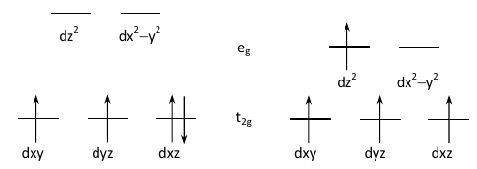
\includegraphics[width=.9\linewidth]{../img/1.png}
\end{center}
同理 d\textsuperscript{6}中央离子在正八面体配位场中的电子结构,在强场中有下图A中的电
子排布,在弱场中有下图B的电子排布。强场络合物因未配对电子少属于低自旋络合物
(共价配键) ,弱场络合物因未配对电子多属于高自旋络合物(电价配键)。
\begin{center}
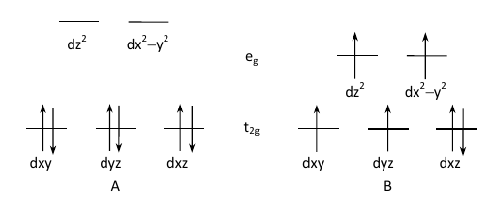
\includegraphics[width=.9\linewidth]{../img/2.png}
\end{center}


\chapter{磁化率的测量}
\label{sec:orgfffe0d2}
测定磁化率的方法很多,有兴趣者可参考文献\textsubscript{[2]}。本实验采用古埃天平测定物质的 X\textsubscript{M}。
本实验的装置图如图所示。将圆柱形样品物质悬挂在天平的一个臂上,使样
品的底部处于电磁铁的中心,即磁场强度最强处。样品应足够长,使其上端顶部的磁场为零。
这样圆柱形样品就处在一不均匀的磁场中,沿样品轴心方向Z存在一磁场强度梯度\(\frac{\partial H}{\partial z}\) ,则作用于样品的力:
\[
f=\left|\int_{H}{O}(X-X_{空})AH\frac{\partial H}{\partial z}dz\right|
\]
式中:A 为样品截面积;X 空为空气的磁化率,H 为磁场强度。如忽略空气的磁化率,则:
\[
f=\left|\int_{H}{O}XAH\frac{\partial H}{\partial z}dz\right|=\frac{1}{2}XH^{2}A
\]
由天平称得装有被测样品的样品管和不装样品的空样品管在加与不加磁场时重量变化
\(\Delta\) W 求出:
\[
f_{1}=\Delta W_{空管}\cdot g
\]
\[
f_{2}=\Delta W_{样品+空管}\cdot g
\]
式中:
\[
\Delta W_{空管}=W_{空管+磁场}-W_{空管}
\]
\[
\Delta W_{样品+空管}=W_{样品+空管+磁场}-W_{样品+空管}
\]
式中 W\textsubscript{空管}为不加磁场时空样品管的质量, W\textsubscript{样品+空管}为装有样品的样品管不加磁场时的质量。
显然,不均匀磁场作用样品的力 \(f = f_{2}-f_{1}\) ,于是有:
\[
\frac{1}{2}XH^{2}A=(\Delta W_{样品+空管}-W_{空管})g
\]
整理后得:
\[
X=\frac{2(\Delta W_{样品+空管}-\Delta W_{空管})g}{H^{2}\cdot A}
\]
由于:
\[
X_{M}=\frac{MX}{\rho}
\]
\[
\rho=\frac{W}{h\cdot A}
\]
则:
\[
X_{M}=\frac{2(\Delta W_{样品+空管}-\Delta W_{空管})ghM}{WH^{2}}
\]
式中 h 为样品高度,W 为样品重量,M 为样品克分子量。
在天平上测出 W,\(\Delta\) W,H,用直尺测出 h,查出 M,g 取 981cm/s\textsuperscript{2} 则可算出 X\textsubscript{M};有:
\[
n(n+2)=\frac{3KT}{N_{O}\beta^{2}}X_{M}
\]
即可推算出样品物质中未成对电子数 n。

磁场强度可用 CT5 型高斯计测出,或用已知克磁化率的莫尔氏盐进行间接标定。
\[
X_{m}=\frac{9500}{T+1}\times 10^{-6}
\]
\part{实验部分}
\label{sec:orgf3f971a}
\chapter{实验仪器与试剂}
\label{sec:org4748c7a}
\begin{center}
\begin{tabular}{lll}
仪器 & 数目 & 试剂\\
\hline
古埃磁天平(磁场,电光天平,励磁电源等) & 一台 & (NH\textsubscript{4})\textsubscript{2}SO\textsubscript{4}\(\cdot\) FeSO\textsubscript{4}\(\cdot\) 6H\textsubscript{2}O\\
CT5 型高斯计(未用到) & 一台 & FeSO\textsubscript{4}\(\cdot\) 7H\textsubscript{2}O\\
软质玻璃样品管 & 4根 & K\textsubscript{4}Fe(CN)\textsubscript{6}\(\cdot\) 3H\textsubscript{2}O\\
装样品工具(研钵,角匙,小漏斗,玻璃棒) & 一套 & \\
\end{tabular}
\end{center}

\chapter{实验步骤}
\label{sec:org19e38f1}
\section{仪器调试(已经提前调好)}
\label{sec:org3ee9441}
    将电压电流调节器旋钮反时针方向旋到底,这时方可打开电源开关。将电
压电流调节旋钮慢慢向顺时针方向旋转,让电流逐渐升至 2A 预热 2 分钟后,磁天平方可使
用。在以后的使用中,通过电压电流调节器,调节电流时要平稳、缓慢,以防因升高或降低
电流太快而损坏晶体管元件。
测准磁场强度是本实验的重要步骤。先对 CT5 高斯计机械调零。校准和各使用档调零。
其方法如下:
\begin{enumerate}
\item 机械调零:在未开机前,旋钮离开“关”指向任何一档,旋动表盖中央调零器凹槽,使指针准指 0 位线(教师已调好)。
\item 校准:开通电源,量程旋钮指示“校准”档,预热 5 分钟,调节右下首“校准”凹槽,使指针准指“校准”线。
\item 放大器 0 位调节,量程旋钮指示“0”档,调节右下首“0”孔中凹槽,使指针指 0 位线。
\item “调零”调节:先将量程旋钮指示“50”档,旋转“调零”旋钮,使指针准批“0”位线。再将量程旋钮指示到需要测量的量限上, (本实验用 1K 档),重新调节“调零”旋钮,使指针指“0”位线。这时方可进行磁场测量。
\end{enumerate}

测量时将霍尔变送器垂直地放入磁极中,使距变送器顶端 3-4mm
处的测量元件位于磁场磁极中心磁场最大值的地方,可稍微平移和转动霍尔探头,使高斯计
的指针指在最大值的方法来确定。如高斯计指针反向,只须将探头转动 180\textsuperscript{\^{}}方可。

\section{磁场两极中心处磁场强度 H 的测定}
\label{sec:org2d03d0b}
\begin{enumerate}
\item 用高斯计重复测量五次,分别读取励磁电流值(本实验用 I\textsubscript{1} = 3A,I\textsubscript{2} = 4A)和对应的磁场强度值。(实际上没有进行此步骤)

\item 用已知 X\textsubscript{m} 的莫尔氏盐标定对应于励磁电流 3A 和 4A 的磁场强度。标定步骤如下:
\end{enumerate}

    将电流调至 0A,取一支清洁、干燥的空样品管悬挂在古埃磁天平的挂钩上,使样品
管底部正好与磁极中心线齐平。准确称得空样品管重量;然后将励磁电流由小至大调节至
1A,迅速且准确地称取此时空样品管的重量;继续由小至大分别调节励磁电流至 2A、3A、
4A 再称重量;继续将励磁电流升至 5A,接着又将励磁电流缓降至 4A,再称空样品管重量;
又将励电流由大至小分别降至 3A、2A、1A,分别再称重量;将励磁电流降至零,又称取一
次样品管重量。上述数据按下表记录。
\begin{center}
\begin{tabular}{llll}
空样品管 & W(增大) & W(减小) & W(平均)\(\Delta\) W\\
\hline
0A &  &  & \\
1A &  &  & \\
2A &  &  & \\
3A &  &  & \\
4A &  &  & \\
\end{tabular}
\end{center}

上述励磁电流由小至大,再由大至小的测量方法,是为了抵消实验时磁场剩磁现象的影
响。此外实验时还须避免气流对测量的影响,并注意勿使样品管与磁极相碰,磁极距离不得
随意变动,每次称量后应将天平托起。

同法重复测定一次,将二次测得的数据取平均值。

取下样品管,将事先研细的莫尔氏盐通过小漏斗装入样品管,在装填时须不断将样品
管底部敲击皮垫,务使粉末样品均匀填实,直至装满约 15 厘米高。用直尺准确量取样品高
度 h。同上法,将装有莫尔氏盐的样品管置于古埃天平的挂钩上,在 0A、1A、2A、3A、4A、
(5A) 、4A、3A、2A、1A、0A 电流下进行称量。测量两次,取两次数据的平均值。测定完
毕,将样品管中的莫尔氏盐倒入回收瓶中,然后洗净、干燥备用。

\section{测定 FeSO\textsubscript{4}\(\cdot\) 7H\textsubscript{2}O 和 K\textsubscript{4}Fe(CN)\textsubscript{6}\(\cdot\) 3H\textsubscript{2}O 的摩尔磁化率}
\label{sec:org8cab36a}
重复以上操作,装入测定样品,重复上述的实验步骤。

\chapter{结果分析与讨论}
\label{sec:org9fa68da}
\section{实验结果}
\label{sec:org05eb916}
   FeSO\textsubscript{4}\(\cdot\) 7H\textsubscript{2}O 的未成对儿电子数为 4,中心原子 Fe\textsuperscript{2+}与六个水分子形成 sp\textsuperscript{3}d\textsuperscript{2} 型配键。
FeSO\textsubscript{4}\(\cdot\) 7H\textsubscript{2}O 是弱场高自旋的电价配键型配合物。

K\textsubscript{4}Fe(CN)\textsubscript{6}\(\cdot\) 3H\textsubscript{2}O 的未成对儿电子数分别为 0,中心原子 Fe\textsuperscript{2+}与 6 个氰根离子形成 d\textsuperscript{2}sp\textsuperscript{3}型
配键。K\textsubscript{4}Fe(CN)\textsubscript{6}\(\cdot\) 3H\textsubscript{2}O 是强场低自旋的共价配键型配合物。

\section{实验讨论}
\label{sec:orge4cb55b}
\begin{enumerate}
\item 对图表的说明及实验结果讨论
\label{sec:org6892176}
\begin{enumerate}
\item 在实验数据测量时,我们采用了励磁电流由小至大,再由大至小的测量方法。在处理数据时,我们将励磁电流由小至大和由大至小的测量数据取平均值,可以抵消实验时磁场剩磁现象的影响,使测量结果更加精准。
\item 由于从高斯计上读出的磁场大小数值不是非常准确,有时示数会跳动,因而我们采用已知克磁化率表达式的莫尔氏盐进行间接标定。这样我们得到的磁场大小数值会更加准确
\item 因为装样品的玻璃管在制造的过程中很难确保玻璃中没有掺杂杂质(而这些杂质中很可能含有某些有磁化率的物质)。为了避免玻璃管对测量的影响,我们先测量一遍玻璃管磁化率,再测量样品的磁化率。这样可以确保我们最终算得的磁化率就是样品本身的磁化率,不受其他因素的影响
\end{enumerate}
\item 误差分析
\label{sec:orgce2e4ac}
     根据公式:
     \[
     n(n+2)=\frac{3KT}{N_{O}\beta^{2}}X_{M}=28.17
     \]
实际算得的 n 值应等于 4.401,与正确值 4 相差较大

相对误差:
\[
\frac{4.401-4}{4}=10.03\%
\]
本次实验的误差较大,本次试验的误差主要来源于三大方面:实验误差、仪器误
差和数据处理误差
\begin{enumerate}
\item 数据处理误差
\label{sec:org13da091}
\begin{enumerate}
\item 首先,实验原理中所给出的数据处理方法中存在着一些近似处理,比如忽略空气的磁化率虽然这些处理并不会对最终结果造成很大的影响,但是,这却必然会给实验结果带来误差。
\item 本实验中处理数据较为复杂,很多步骤中都有数据的舍入误差。
\end{enumerate}
\item 仪器误差
\label{sec:orgaf20341}
\begin{enumerate}
\item 本实验所使用的古埃磁天平仪器误差较大。在实验中,读数会跳动,而且有时会有读数滞后的现象发生。
\item 本实验中测量的物质的重量变化很小, 而只要稍微碰触到磁天平读数就会变化。外界环境条件对于重量的读数值影响很大。
\end{enumerate}
\item 实验误差
\label{sec:orgad36527}
\begin{enumerate}
\item 本实验所使用的样本管已被反复使用多次,在这反复使用的过程中,难免会被污染而致使其纯度不够。这会较大程度地影响实验的准确性。
\item 本实验所使用的三种样品中均含有二价铁离子,它具有还原性,在空气中是比较容易被氧化的。在研磨的过程中尤其容易被氧化.
\item 实验中,励磁电流不能每次都准确地定在同一位置,虽然示数一致,但实际旋转的度数不尽相同
\item 装样品时我们很难将样品完全压平,尤其是最上面的那一部分。所以,我们测得的样品高度是有误差的
\end{enumerate}
\item 对实验的体会和认识
\label{sec:orge6b64fd}
\begin{enumerate}
\item 本实验中所需要的一部分理论知识是自己之前没有接触过的,原理公式的推导中也有一些新的方法。通过这次实验,我也进一步了解了这些方法。
\item 本实验中,我们通过对于宏观量的测量得到了物质微观结构上的一些特征。
\item 在涉及到有关磁性质的测量时,往往会出现剩磁现象,因此,我们在测量时要将磁场由大变小和由小变大各测量一次。
\end{enumerate}
\end{enumerate}
\end{enumerate}

\part{参考文献}
\label{sec:org33f6a67}
\begin{enumerate}
\item 傅献彩 沈文霞 姚天扬.物理化学.北京:高等教育出版社,2006.
\item 崔献英 柯燕雄 单绍纯.物理化学实验.合肥:中国科学技术大学出版社,2000.
\item 《物理化学讲义之结构化学实验》 中科大 物理化学实验组
\item 《络合物的磁化率测定实验数据处理的改进》 李玉玲 曹丰璞 南阳师范学院学报 2010 年 3 月 第 9 卷第 3 期
\item 《物质结构》(第二版)P316 潘道皑 赵成大 等主编 高等教育出版社 2006年印刷
\item 《络合物电子结构的测定——古埃磁天平法(磁化率的测定)实验方法的讨论》 黄桂萍 张菊芳 叶丽莎 江西化工 2008 年第 1 期
\end{enumerate}

\part{附录: 数据处理过程}
\label{sec:orgb25180f}
\chapter{原始记录}
\label{sec:orgddd2cb3}
如管中有填充物,其高度为约15cm.   
\section{管1}
\label{sec:orgc0afecb}
\begin{enumerate}
\item 空管 (21.8\textsuperscript{\^{}}C)
\label{sec:org8e47d1d}
\begin{center}
\begin{tabular}{rrrrrrr}
I(A) & W\textsubscript{1}(\(\uparrow\))(g) & W\textsubscript{1}(\(\downarrow\))(g) & W\textsubscript{2}(\(\uparrow\))(g) & W\textsubscript{2}(\(\downarrow\))(g) & \overline{W}(g) & \(\Delta\) W(g)\\
\hline
0.0 & 14.3883 & 14.3888 & 14.3888 & 14.3887 & 14.38865 & 0.00000\\
0.1 & 14.3884 & 14.3888 & 14.3887 & 14.3886 & 14.38863 & -0.00002\\
0.2 & 14.3885 & 14.3886 & 14.3886 & 14.3885 & 14.38855 & -0.00010\\
0.3 & 14.3884 & 14.3883 & 14.3885 & 14.3884 & 14.38840 & -0.00025\\
0.4 & 14.3881 & 14.3881 & 14.3882 & 14.3882 & 14.38815 & -0.00050\\
\end{tabular}
\end{center}

\begin{center}
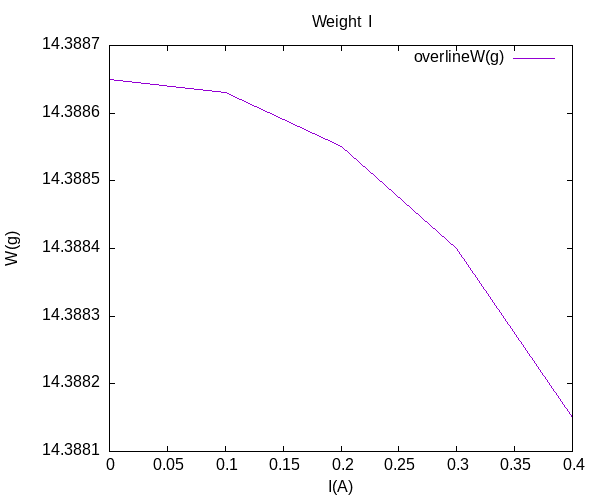
\includegraphics[width=.9\linewidth]{../img/1-1.png}
\end{center}
\item 亚铁氰化钾(s) (23.37\textsuperscript{\^{}}C,6.50543g)
\label{sec:org2207ebb}
\begin{center}
\begin{tabular}{rrrrrrr}
I(A) & W\textsubscript{1}(\(\uparrow\))(g) & W\textsubscript{1}(\(\downarrow\))(g) & W\textsubscript{2}(\(\uparrow\))(g) & W\textsubscript{2}(\(\downarrow\))(g) & \overline{W}(g) & \(\Delta\) W(g)\\
\hline
0.0 & 20.8940 & 20.8941 & 20.8941 & 20.8941 & 20.89408 & 0.00000\\
0.1 & 20.8940 & 20.8940 & 20.8940 & 20.8941 & 20.89403 & -0.00005\\
0.2 & 20.8939 & 20.8938 & 20.8939 & 20.8939 & 20.89388 & -0.00020\\
0.3 & 20.8936 & 20.8935 & 20.8937 & 20.8937 & 20.89363 & -0.00045\\
0.4 & 20.8933 & 20.8931 & 20.8934 & 20.8933 & 20.89328 & -0.00080\\
\end{tabular}
\end{center}
\begin{center}
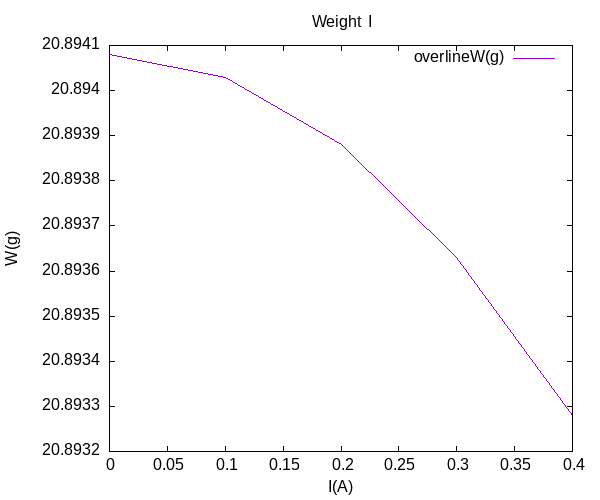
\includegraphics[width=.9\linewidth]{../img/1-2.png}
\end{center}
\item 亚铁氰化钾(aq) (23.37\textsuperscript{\^{}}C)
\label{sec:org2450f60}
\begin{center}
\begin{tabular}{rrrrrrr}
I(A) & W\textsubscript{1}(\(\uparrow\))(g) & W\textsubscript{1}(\(\downarrow\))(g) & W\textsubscript{2}(\(\uparrow\))(g) & W\textsubscript{2}(\(\downarrow\))(g) & \overline{W}(g) & \(\Delta\) W(g)\\
\hline
0.0 & 21.0581 & 21.0568 & 21.0566 & 21.0562 & 21.05693 & 0.00000\\
0.1 & 21.0577 & 21.0569 & 21.0566 & 21.0561 & 21.05683 & -0.00010\\
0.2 & 21.0574 & 21.0568 & 21.0564 & 21.0559 & 21.05663 & -0.00030\\
0.3 & 21.0570 & 21.0565 & 21.0562 & 21.0557 & 21.05635 & -0.00058\\
0.4 & 21.0565 & 21.0563 & 21.0557 & 21.0554 & 21.05598 & -0.00095\\
\end{tabular}
\end{center}
\begin{center}
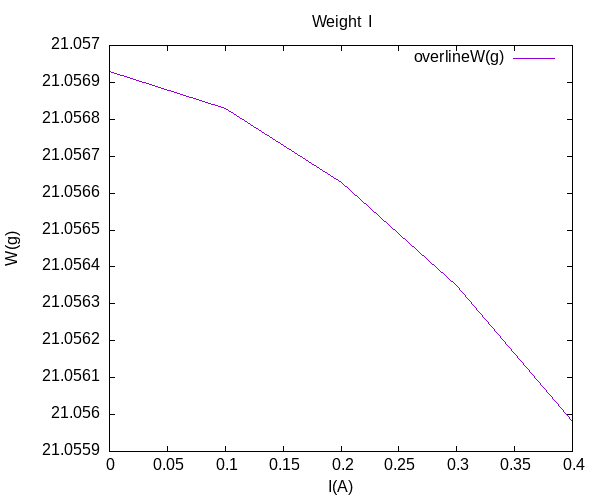
\includegraphics[width=.9\linewidth]{../img/1-3.png}
\end{center}
\end{enumerate}
\section{管2}
\label{sec:org7a2aa35}
\begin{enumerate}
\item 空管 (23.05\textsuperscript{\^{}}C)
\label{sec:org31b3e9a}
\begin{center}
\begin{tabular}{rrrrrrr}
I(A) & W\textsubscript{1}(\(\uparrow\))(g) & W\textsubscript{1}(\(\downarrow\))(g) & W\textsubscript{2}(\(\uparrow\))(g) & W\textsubscript{2}(\(\downarrow\))(g) & \overline{W}(g) & \(\Delta\) W(g)\\
\hline
0.0 & 14.8300 & 14.8299 & 14.8299 & 14.8299 & 14.82993 & 0.00000\\
0.1 & 14.8299 & 14.8299 & 14.8299 & 14.8299 & 14.82990 & -0.00003\\
0.2 & 14.8299 & 14.8298 & 14.8299 & 14.8298 & 14.82985 & -0.00008\\
0.3 & 14.8297 & 14.8297 & 14.8298 & 14.8296 & 14.82970 & -0.00023\\
0.4 & 14.8296 & 14.8295 & 14.8295 & 14.8294 & 14.82950 & -0.00043\\
\end{tabular}
\end{center}
\begin{center}
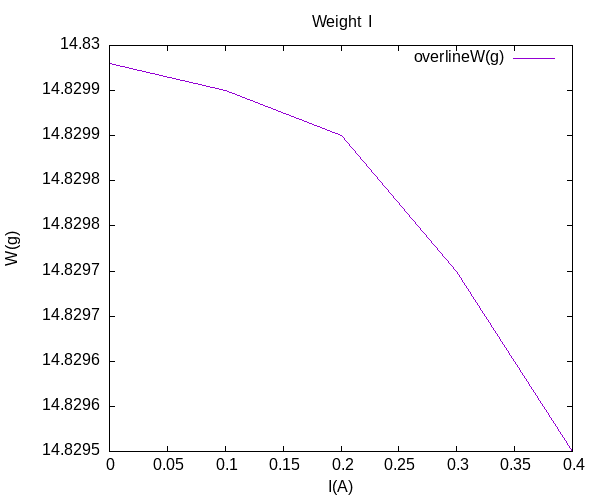
\includegraphics[width=.9\linewidth]{../img/2-1.png}
\end{center}
\item 硫酸亚铁(s) (23.56\textsuperscript{\^{}}C,6.62997g)
\label{sec:org7fd666c}
\begin{center}
\begin{tabular}{rrrrrrr}
I(A) & W\textsubscript{1}(\(\uparrow\))(g) & W\textsubscript{1}(\(\downarrow\))(g) & W\textsubscript{2}(\(\uparrow\))(g) & W\textsubscript{2}(\(\downarrow\))(g) & \overline{W}(g) & \(\Delta\) W(g)\\
\hline
0.0 & 21.4599 & 21.4599 & 21.4599 & 21.4599 & 21.45990 & 0.00000\\
0.1 & 21.4620 & 21.4617 & 21.4621 & 21.4620 & 21.46195 & 0.00205\\
0.2 & 21.4676 & 21.4683 & 21.4675 & 21.4679 & 21.46783 & 0.00793\\
0.3 & 21.4769 & 21.4781 & 21.4769 & 21.4781 & 21.47750 & 0.01760\\
0.4 & 21.4903 & 21.4911 & 21.4908 & 21.4913 & 21.49088 & 0.03098\\
\end{tabular}
\end{center}
\begin{center}
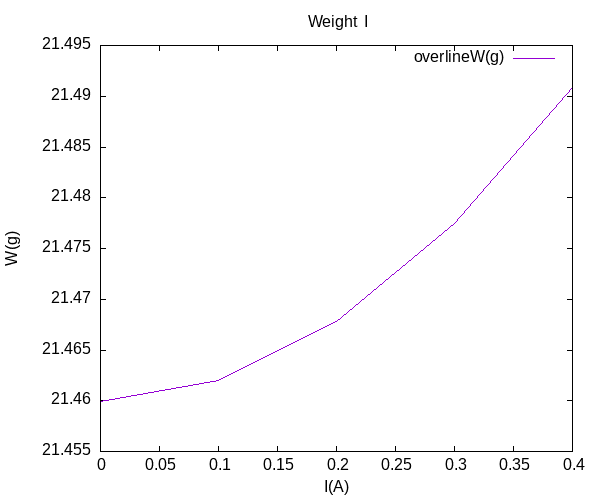
\includegraphics[width=.9\linewidth]{../img/2-2.png}
\end{center}
\item 硫酸亚铁(aq) (23.43\textsuperscript{\^{}}C)
\label{sec:orgfc0d2f1}
\begin{center}
\begin{tabular}{rrrrrrr}
I(A) & W\textsubscript{1}(\(\uparrow\))(g) & W\textsubscript{1}(\(\downarrow\))(g) & W\textsubscript{2}(\(\uparrow\))(g) & W\textsubscript{2}(\(\downarrow\))(g) & \overline{W}(g) & \(\Delta\) W(g)\\
\hline
0.0 & 21.7271 & 21.7268 & 21.7267 & 21.7260 & 21.72665 & 0.00000\\
0.1 & 21.7277 & 21.7274 & 21.7272 & 21.7269 & 21.72730 & 0.00065\\
0.2 & 21.7295 & 21.7295 & 21.7291 & 21.7290 & 21.72928 & 0.00263\\
0.3 & 21.7329 & 21.7328 & 21.7322 & 21.7322 & 21.73253 & 0.00588\\
0.4 & 21.7375 & 21.7373 & 21.7365 & 21.7369 & 21.73705 & 0.01040\\
\end{tabular}
\end{center}
\begin{center}
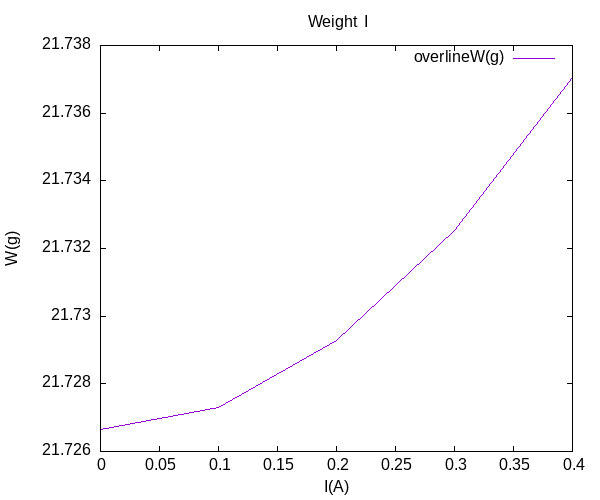
\includegraphics[width=.9\linewidth]{../img/2-3.png}
\end{center}
\end{enumerate}
\section{管3}
\label{sec:orgb9e82cb}
\begin{enumerate}
\item 空管 (23.28\textsuperscript{\^{}}C)
\label{sec:orga520ca2}
\begin{center}
\begin{tabular}{rrrrrrr}
I(A) & W\textsubscript{1}(\(\uparrow\))(g) & W\textsubscript{1}(\(\downarrow\))(g) & W\textsubscript{2}(\(\uparrow\))(g) & W\textsubscript{2}(\(\downarrow\))(g) & \overline{W}(g) & \(\Delta\) W(g)\\
\hline
0.0 & 13.9477 & 13.9477 & 13.9477 & 13.9480 & 13.94778 & 0.00000\\
0.1 & 13.9478 & 13.9476 & 13.9475 & 13.9478 & 13.94768 & -0.00010\\
0.2 & 13.9476 & 13.9476 & 13.9476 & 13.9477 & 13.94763 & -0.00015\\
0.3 & 13.9475 & 13.9475 & 13.9475 & 13.9476 & 13.94753 & -0.00025\\
0.4 & 13.9471 & 13.9474 & 13.9473 & 13.9473 & 13.94728 & -0.00050\\
\end{tabular}
\end{center}
\begin{center}
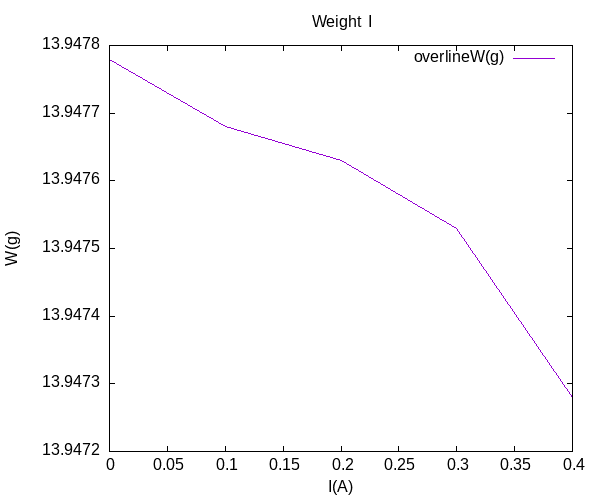
\includegraphics[width=.9\linewidth]{../img/3-1.png}
\end{center}
\item 莫尔盐(s) (23.62\textsuperscript{\^{}}C,6.75692g)
\label{sec:org5acdc6d}
\begin{center}
\begin{tabular}{rrrrrrr}
I(A) & W\textsubscript{1}(\(\uparrow\))(g) & W\textsubscript{1}(\(\downarrow\))(g) & W\textsubscript{2}(\(\uparrow\))(g) & W\textsubscript{2}(\(\downarrow\))(g) & \overline{W}(g) & \(\Delta\) W(g)\\
\hline
0.0 & 20.7046 & 20.7047 & 20.7047 & 20.7048 & 20.70470 & 0.00000\\
0.1 & 20.7060 & 20.7064 & 20.7062 & 20.7066 & 20.70630 & 0.00160\\
0.2 & 20.7103 & 20.7108 & 20.7103 & 20.7108 & 20.71055 & 0.00585\\
0.3 & 20.7176 & 20.7183 & 20.7173 & 20.7182 & 20.71785 & 0.01315\\
0.4 & 20.7273 & 20.7275 & 20.7275 & 20.7279 & 20.72755 & 0.02285\\
\end{tabular}
\end{center}
\begin{center}
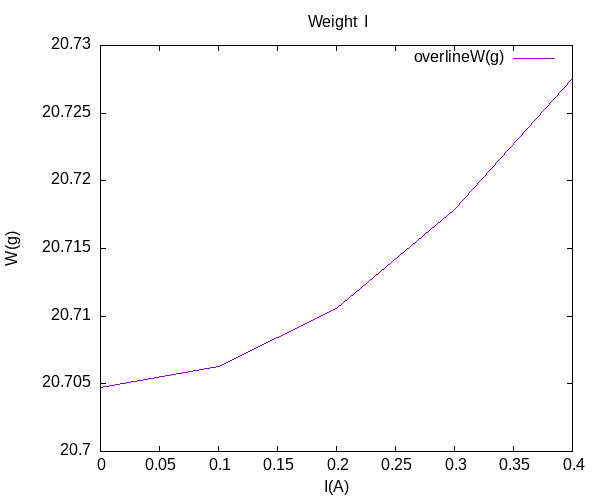
\includegraphics[width=.9\linewidth]{../img/3-2.png}
\end{center}
\item 莫尔盐(aq) (23.56\textsuperscript{\^{}}C)
\label{sec:org6b8623c}
\begin{center}
\begin{tabular}{rrrrrrr}
I(A) & W\textsubscript{1}(\(\uparrow\))(g) & W\textsubscript{1}(\(\downarrow\))(g) & W\textsubscript{2}(\(\uparrow\))(g) & W\textsubscript{2}(\(\downarrow\))(g) & \overline{W}(g) & \(\Delta\) W(g)\\
\hline
0.0 & 20.5646 & 20.5631 & 20.5631 & 20.5619 & 20.56318 & 0.00000\\
0.1 & 20.5646 & 20.5633 & 20.5632 & 20.5621 & 20.56330 & 0.00012\\
0.2 & 20.5651 & 20.5644 & 20.5639 & 20.5633 & 20.56418 & 0.00100\\
0.3 & 20.5664 & 20.5660 & 20.5652 & 20.5650 & 20.56565 & 0.00247\\
0.4 & 20.5686 & 20.5685 & 20.5673 & 20.5672 & 20.56790 & 0.00472\\
\end{tabular}
\end{center}
\begin{center}
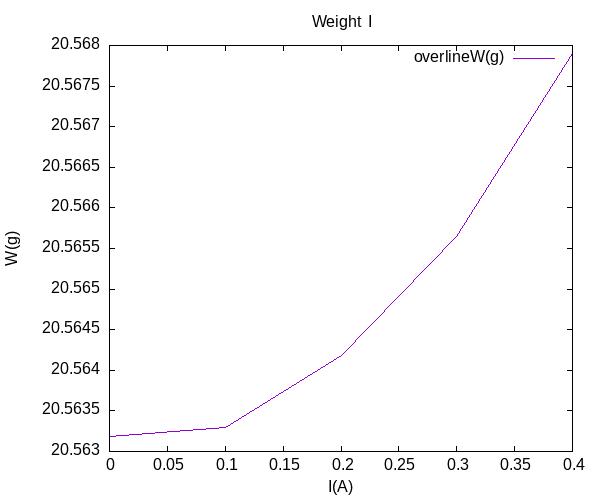
\includegraphics[width=.9\linewidth]{../img/3-3.png}
\end{center}
\end{enumerate}
\chapter{数据处理}
\label{sec:orgbb7fc1b}
\section{由莫尔盐磁化率计算磁场强度}
\label{sec:org256244c}
室温T=273.15K+23.62\textsuperscript{\^{}}C =296.77K,由公式:
\[
X_{m}=\frac{9500}{T+1}\times 10^{-6}
\]
得到莫尔氏盐的克磁化率和摩尔磁化率为:
\[
X_{m}=3.1904\times 10^{-5}cm^{3}/g
\]
由公式:
\[
X_{M}=\frac{2(\Delta W_{样品+空管}-\Delta W_{空管})ghM}{WH^{2}}=\frac{2(\Delta m_{1}-\Delta m_{0})ghM}{mH^{2}}
\]
将测得的数据依次代入,其中式中 h 为样品高度 h=15.0cm,W 为样品重量 6.75692g,M 为样品克分子量 392.14g/mol,g=981cm/s2:
\begin{center}
\begin{tabular}{rrrr}
I(A) & \(\Delta\) m\textsubscript{s}(g) & \(\Delta\) m\textsubscript{空}(g) & H(Gauss)\\
\hline
0.1 & 0.00160 & -0.00010 & 481.751\\
0.2 & 0.00585 & -0.00015 & 905.053\\
0.3 & 0.01315 & -0.00025 & 1352.541\\
0.4 & 0.02285 & -0.00050 & 1785.425\\
\end{tabular}
\end{center}

\section{样品磁化率及孤电子对的计算}
\label{sec:org1e524dc}
在下面的计算中,均将将数据代入:
\[
    X_{M}=\frac{2(\Delta W_{样品+空管}-\Delta W_{空管})ghM}{WH^{2}}
    \]
\begin{enumerate}
\item 硫酸亚铁(23.56\textsuperscript{\^{}}C,6.62997g)
\label{sec:org9b0597a}
\begin{center}
\begin{tabular}{rrrrr}
I(A) & \(\Delta\) m\textsubscript{s}(g) & \(\Delta\) m\textsubscript{空}(g) & H(Gauss) & X\textsubscript{m}(cm\textsuperscript{3}/mol)\\
\hline
0.1 & 0.00205 & -0.00003 & 481.751 & 0.011060\\
0.2 & 0.00793 & -0.00008 & 905.053 & 0.012068\\
0.3 & 0.01760 & -0.00023 & 1352.541 & 0.012028\\
0.4 & 0.03098 & -0.00043 & 1785.425 & 0.012160\\
\end{tabular}
\end{center}
X\textsubscript{m}平均值为:0.011829

又
\[
n(n+2)=\frac{3KT}{N_{O}\beta^{2}}X_{M}
\]
(N\textsubscript{O} = 6.023\texttimes{} 10\textsuperscript{23},K = 1.386\texttimes{} 10\textsuperscript{-16} 尔格/度,\(\beta\) = 9.274\texttimes{} 10\textsuperscript{-21}尔格/高斯)
\[
n(n+2)=28.17
\]
算得n=4.401,取整数,n=4

\item 亚铁氰化钾(23.37\textsuperscript{\^{}}C,6.50543g)
\label{sec:org10db2f7}
\begin{center}
\begin{tabular}{rrrrr}
I(A) & \(\Delta\) m\textsubscript{s}(g) & \(\Delta\) m\textsubscript{空}(g) & H(Gauss) & X\textsubscript{m}(cm\textsuperscript{3}/mol)\\
\hline
0.1 & -0.00005 & -0.00002 & 481.751 & -0.000247\\
0.2 & -0.00020 & -0.00010 & 905.053 & -0.000233\\
0.3 & -0.00045 & -0.00025 & 1352.541 & -0.000209\\
0.4 & -0.00080 & -0.00050 & 1785.425 & -0.000180\\
\end{tabular}
\end{center}
X\textsubscript{m}平均值为:0.000217
又
\[
n(n+2)=\frac{3KT}{N_{O}\beta^{2}}X_{M}
\]
(N\textsubscript{O} = 6.023\texttimes{} 10\textsuperscript{23},K = 1.386\texttimes{} 10\textsuperscript{-16} 尔格/度,\(\beta\) = 9.274\texttimes{} 10\textsuperscript{-21}尔格/高斯)
\[
n(n+2)=-0.50
\]
算得n=-0.3,取整数,n=0
\end{enumerate}
\section{讨论 FeSO\textsubscript{4}\(\cdot\) 7H\textsubscript{2}O 和K\textsubscript{4}Fe(CN)\textsubscript{6}\(\cdot\) 3H\textsubscript{2}O 的 Fe\textsuperscript{2+}的最外层电子结构和配键类型}
\label{sec:org6cb9ccb}
\begin{itemize}
\item FeSO\textsubscript{4}\(\cdot\) 7H\textsubscript{2}O 未成对电子数 n=4,Fe\textsuperscript{2+} 最外层电子排布为 3d\textsuperscript{6},推断 FeSO\textsubscript{4}\(\cdot\) 7H\textsubscript{2}O中Fe\textsuperscript{2+}最外层电子结构为:
\begin{center}
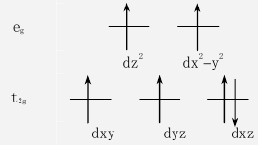
\includegraphics[width=.9\linewidth]{../img/3.png}
\end{center}
\item K\textsubscript{4}Fe(CN)\textsubscript{6}\(\cdot\) 3H\textsubscript{2}O 未成对电子数 n=0,Fe\textsuperscript{2+}最外层电子排布为 3d\textsuperscript{6},推断 K\textsubscript{4}Fe(CN)\textsubscript{6}\(\cdot\) 3H\textsubscript{2}O 中 Fe\textsuperscript{2+}最外层电子结构为:
\end{itemize}
\begin{center}
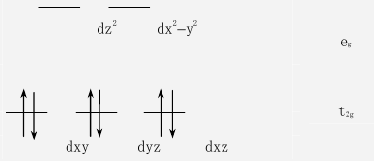
\includegraphics[width=.9\linewidth]{../img/4.png}
\end{center}
\end{document}
